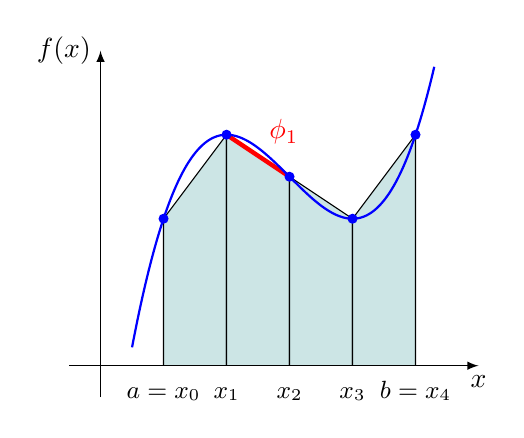
\begin{tikzpicture}[scale=0.8] % ,declare function={f(\x)=((1/3)*(\x)^(3)-3*(\x)^(2)+8*\x-3;}]

\pgfmathdeclarefunction{f}{1}{%
    \pgfmathparse{((1/3)*(#1)^(3)-3*(#1)^(2)+8*#1-3}%
}
\coordinate (start) at (.8,{f(.8)});
\coordinate (x0) at (1,{f(1)});
\coordinate (x1) at (2,{f(2)});
\coordinate (x2) at (3,{f(3)});
\coordinate (x3) at (4,{f(4)});
\coordinate (x4) at (5,{f(5)});
\coordinate (end) at (5.05,{f(5.05)});

\draw[fill=teal!20!white] (1,0)--(1,{f(1)})--(2,{f(2)})--(2,0);
\draw[fill=teal!20!white] (2,0)--(2,{f(2)})--(3,{f(3)})--(3,0);
\draw[fill=teal!20!white] (3,0)--(3,{f(3)})--(4,{f(4)})--(4,0);
\draw[fill=teal!20!white] (4,0)--(4,{f(4)})--(5,{f(5)})--(5,0);

\draw[ultra thick, red] (2,{f(2)})--(3,{f(3)}) node[midway,above right] {$\phi_1$};

%\draw (5,0)--(5,{f(5)});
\draw [-latex] (-0.5,0) -- (6,0) node (xaxis) [below] {$x$};
\draw [-latex] (0,-0.5) -- (0,5) node [left] {$f(x)$};
\foreach \x/\xtext in {1/a=x_0 ,2/x_1, 3/x_2 , 4/x_3 , 5/b=x_4}
 \draw[xshift=\x cm] node[below=2pt,fill=white,font=\small, anchor=south, yshift=-5mm] {$\xtext$};
\draw[domain=.5:5.3,samples=200,variable=\x,blue,thick] plot ({\x},{f(\x)});                 
\foreach \n in {0,1,2,3,4}
\draw[blue,fill=blue] (x\n) circle (2pt) node[font=\normalsize] {$ $};    
% \draw[latex-latex] (2,1)--(3,1) node[midway, anchor=south] {$\frac{b-a}{p}$};      
\end{tikzpicture}